Waste management is a constant issue, that is dealt with on the daily by different organisations.
According to Eurostat, the countries in Europe have had a rather stable production of waste in the past decade. In 2014, over 200 million tonnes of waste have been generated just by households in european countries\cite{eurostat}.
How waste is handled is a highly relevant issue in modern society, and the design of smart garbage systems for both houses and cities can help monitor the situation.

The traditional approach on waste management comes from a logistical point of view.
However, imagine not the amounts nor the location of the bin being the driving force for interacting with it, but rather its smell.

This is essentially the innovative take of our system - smell as an additional parameter.
This additional information can be used in conjunction with existing systems or be used to produce an entirely new experience centered around the waste bin.
Following this concept, a prototype of a simple system has been developed.
With low cost and easily obtainable technology, the system measures both smell and garbage amount directly from the bin.
This information is transmitted from the bin to the cloud and made readily available to a set of client devices.
We use an android application to present the data to the user in two different modes, namely as an ambient display or as a smartphone app.
Figure ~\ref{fig:smartbin} shows an overview of the system.

The system is specifically designed for private use inside a household, but can be easily adjusted and extended for different usages.

In this paper we describe the system specifications and evaluation, and discuss its potential integration in other scenarios different from the one presented.

\begin{figure}
\centering
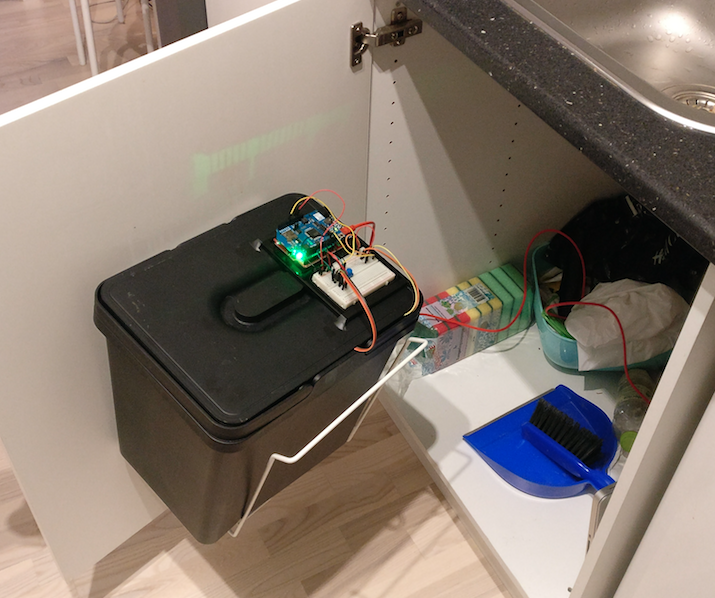
\includegraphics[scale=.2]{img/smartbin}
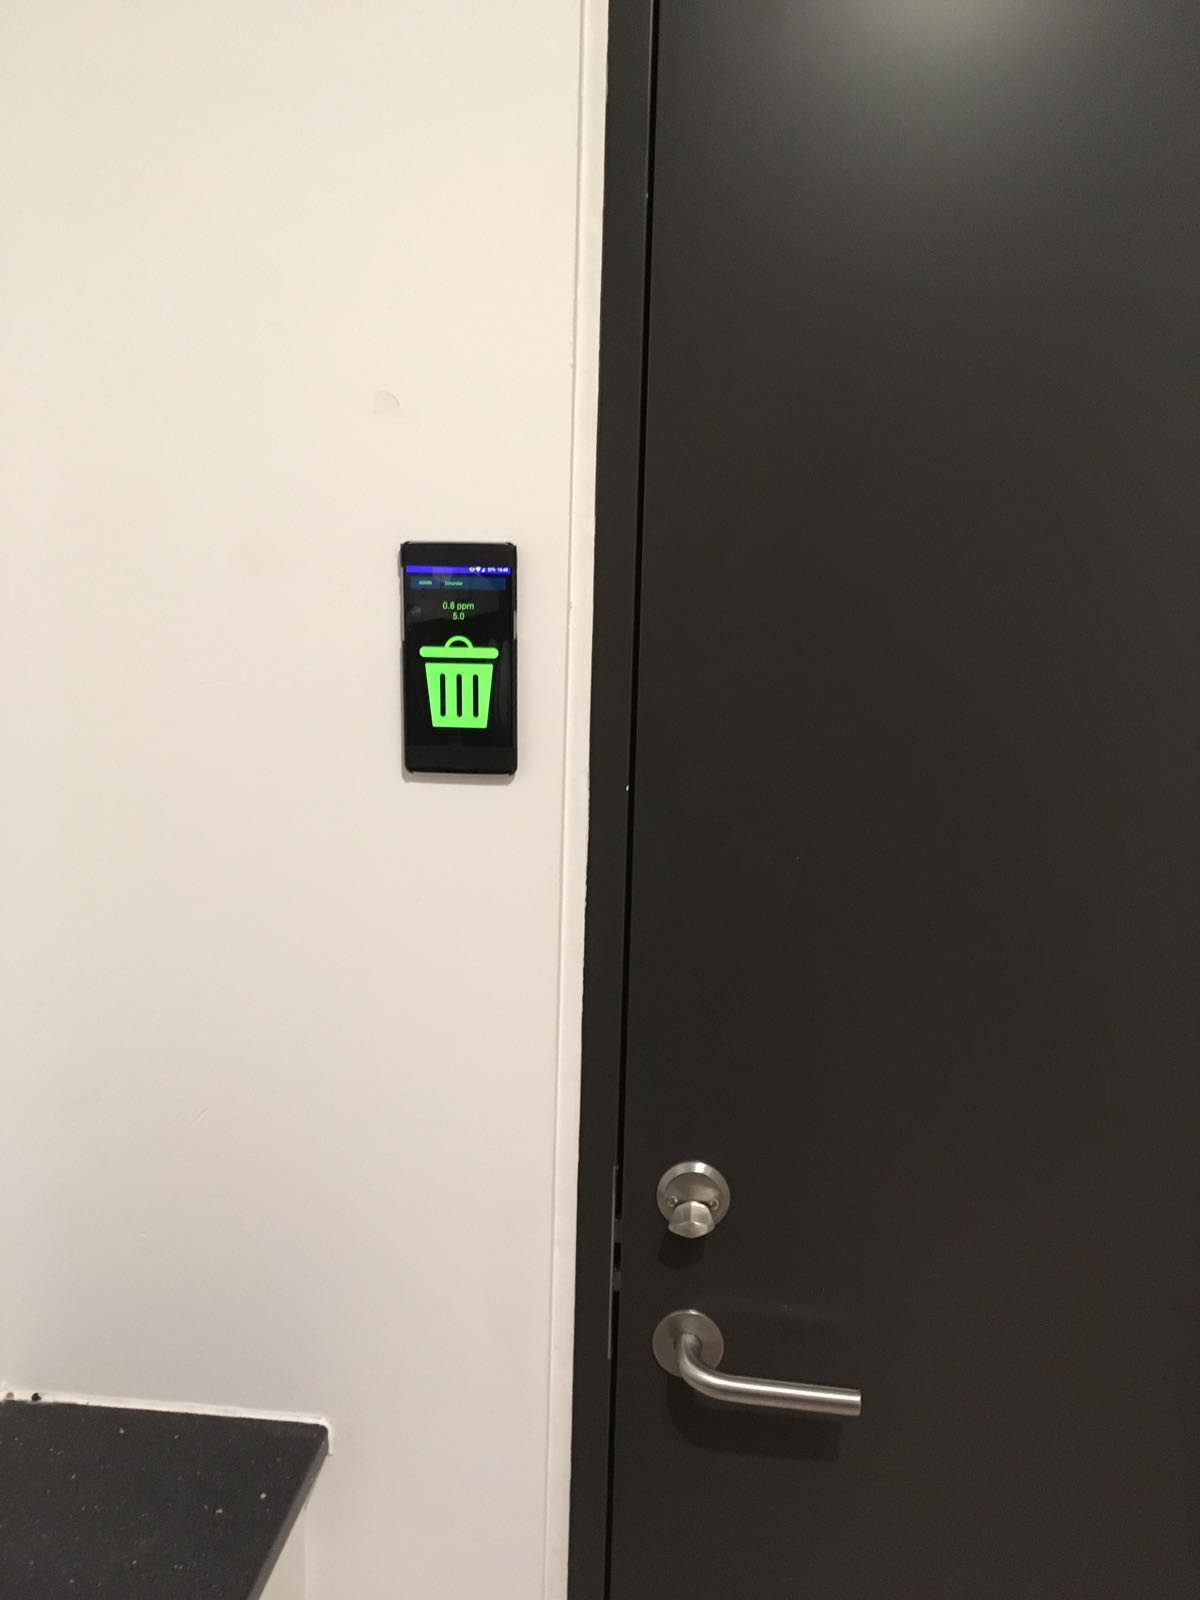
\includegraphics[scale=.075]{img/IMG-20161130-WA0000}
\caption{The SmartBin system overview, the bin with ambient display}
\label{fig:smartbin}
\end{figure}